\section{Opgave 3}
I denne opgave undersøges funktionen $f:\mathbb{R}^2 \rightarrow \mathbb{R}$ givet ved
\begin{align*}
f(x,y) = \frac{5}{4} x^2 y-\frac14 x^4 -y^2+1
\end{align*}
Vi starter med at betragte en kurve $K$ givet ved parameterfremstillingen
\begin{align}
\left[
    \begin{array}{c}
        x\\y
    \end{array}
\right] 
= \textbf{r}(u) = \left(u,\frac12 u^2 \right), u\in \mathbb{R}
\end{align}
\subsection{Lad $h$ betegne den sammensatte funktion $h(u)=f(\textbf{r}(u)),u\in \textbf{R}$. Lav et Maple-plot hvor du har brugt $h$ til at løfte $K$ op på grafen for $f$. Bestem de værdier af $u$ for hvilke $h(u)=1$ og $h'(u)=0$, og angiv de intervaller for $u$ i hvilke $h'(u)$ er negativ, henholdsvis positiv.}

For at plotte funktionen $f(x,y)$ bruges plot3d. Spacecurve bruges til at plotte den sammensatte funktion $h(u)$. Disse funktioner ses i Maple.

Værdierne for $u$ findes ved at lave to ligninger med en ubekendt. Den første ligning er at $h(u)=1$ og $h'(u)=0$. De løses med Maple og $u$ findes til at være 0. Dette ses i Maple.
\begin{align}
    h(u)=1 \text{ og } h'(u)=0 \rightarrow u=0
\end{align}

For at se for hvilke værdier af u hvor $h'(u)$ er negativ plottes funktionen hvor der så ses for hvilket værdier for u at $h'(u)$ er negativ.

\begin{figure}[htp]
    \centering
    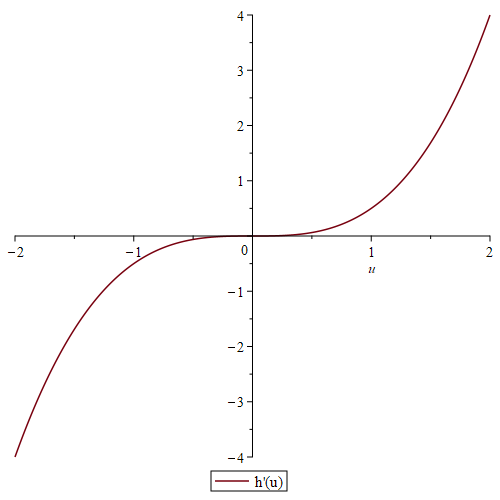
\includegraphics[width=8cm]{diffh.png}
        \caption{$h'(u)$ plottet omkring origo}
    \label{diffh}
\end{figure}

Det ses på figur \ref{diffh}, at når u bliver negativt vil $h'(u)$ også blive negativt og omvendt at når u bliver positivt vil $h'(u)$ også blive positivt


Vi betragter i det følgende punkterne $A = (0,-1)$ og $B=(0,0)$.

\subsection{Bestem Hessematricen for $f$ i $A$, og bestem arten af det approksimerede andengradspolynomium $P_2$ for $f$ med udviklingspunktet $A$. Illustrer. Bestem den største fejl man begår, hvis man benytter $P_2$ i stedet for $f$ på det afsluttende kvadrat der er afgrænset af linjerne $x=\frac{-1}{10},x=\frac{1}{10},y=\frac{-11}{10}$ og $y=\frac{-9}{10}$.}

Hessematricen er bygget op af de dobbelt-differentierede funktioner for $f$ i $A$. 
\begin{align}
    H(x_0,y_0)= 
    \left[
    \begin{array}{cc}
        f^{''}_{xx}(x_0,y_0) & f^{''}_{xy}(x_0,y_0)\\f^{''}_{xy}(x_0,y_0) & f^{''}_{yy}(x_0,y_0)
    \end{array}
\right] 
\end{align}
Hvor $(x_0,y_0)=(0,-1)$.
Dette løses og hessematricen fås til at være:
\begin{align}
    H(x_0,y_0)= 
    \left[
    \begin{array}{cc}
        -\frac{5}{2} & 0\\0 & -2
    \end{array}
\right] 
\end{align}
For at finde det approksimerede andengradspolynomium bruges mtaylor funktionen i maple. Så fås det approksimerede andengradspolynomium til:
\begin{align}
    P2(0,-1) = 1-\frac{5\cdot x^2}{4} - y^2
\end{align}

Denne funktion ligner en elliptisk cylinderflade, hvis ligning har formen:
\begin{align}
    \frac{x^2}{a^2} + \frac{y^2}{b^2} = 1
\end{align}

For at finde den største fejl man begår laves en funktion ud fra den originale funktion $f$ og den approksimerede funktion $P2$. Denne funktion er
\begin{align}
    R(x,y) = f(x,y)-P2(x,y)
\end{align}

Med denne funktion skal der findes extrema for funktion. Dete skal være maksimum og ikke minimum, da den største værdi skal findes. Derfor bruges også den dobbelt differentierede funktion. $R''(x,y)$. 

\subsection{Gør rede for at $B$ er et stationært punkt for $f$ hvor man ikke umiddelbart kan bruge Hessemetoden til at afgøre om $B$ er sted for et lokalt extremum.}

Hvis $B$ er et stationært punkt betyder det at gradientet for punktet vil være lig $(0,0)$.\footnote{Defintion 21.9} Dette testes.
\begin{align}
    \nabla f(0,0) = \left(f'_x(0,0),f'_y(0,0)\right) = (0,0)
\end{align}
Dette betyder at $B$ er et stationært punkt.

Så findes hessematricen for $f$ i $B$, da denne bruges til hessemetoden som kan afgøre om $B$ er et lokalt extremum.

\begin{align}
    H(0,0) = 
    \left[
        \begin{array}{cc}
            0 & 0\\0 & -2
        \end{array}
    \right] 
\end{align}
Heraf aflæses egenværdierne til at være $(0,-2)$.
Dette betyder at hvis man ganger egenværdierne sammen giver det 0. Denne egenskab betyder så at man ikke kan sikre at $B$ er et lokalt extremum ud fra hessemetoden\footnote{Definition 21.17}.



\subsection{Vis at restriktionen af $f$ til alle rette linjer gennem $B$ har lokalt maksimum i $B$. Kan vi på den baggrund slutte at $f$ har lokalt maksimum i $B$? HAR $f$ lokalt maksimum i $B$?}




